\section{Коммуникационная сложность}

В данном разделе мы рассмотрим, как классические коммуникационные задачи и техники, так и применения
теории информаии в коммуникационной сложности.

\begin{definition}
    \deftext{Коммуникационный протокол} для функции $f\colon X \times Y \to Z$~--- это корневое двоичное
    дерево, которое описывает совместное вычисление Алисой и Бобом функции $f$. В этом дереве:
    \begin{itemize}
        \item каждая внутренняя вершина $v$ помечена меткой $a$ или $b$, означающей очередь хода Алисы
            или Боба соответственно;
        \item для каждой вершины, помеченной $a$, определена функция $g_v\colon X \to \{0, 1\}$;
            аналогично, для каждой вершины $v$ с пометкой $b$, определена функция $h_v\colon Y \to \{0,
            1\}$;
        \item каждая внутренняя вершина имеет двух потомков, ребро к первому потомку помечено нулём, а
            ребро ко второму~--- единицей;
        \item каждый лист помечен значением из множества $Z$.
    \end{itemize}

    Пометки $a$ или $b$, означают очередность хода Алисы или Боба соответственно. Функции $g_v$ или $h_v$
    говорят какой бит нужно послать, если вычисление находится в вершине $v$. Таким образом, каждая пара
    входов $(x, y)$ определяет путь от корня до листа в описанном двоичном дереве естественным
    образом. Будем говорить, что коммуникационный протокол \deftext{вычисляет} функцию $f$, если для всех
    пар $(x, y) \in X \times Y $ этот путь заканчивается в листе с пометкой $f(x, y)$.  
    
    \deftext{Коммуникационной сложностью} функции $f$ называется наименьшая глубина протокола,
    вычисляющего функцию $f$. Будем обозначать её символом $\DCC(f)$.
    
    Каждой функции $f$ будем сопоставлять матрицу $X \times Y$, в которой в клетке $(x_i, y_j)$ стоит
    значение $f(x_i, y_j)$.
\end{definition}

Следующая лемма нам описывает комбинаторное свойство коммуникационных протоколов, которое нам позволяет
доказывать нижние оценки.

\begin{proposition} 
    Рассмотрим дерево протокола со входом из множества $X \times Y$. Рассмотрим в нём произвольную
    вершину $u$. Тогда все входы, из которых можно прийти в вершину $u$, образуют прямоугольник
    $R_u \coloneqq X_u \times Y_u \subseteq X \times Y$.
\end{proposition}

\begin{proof}
    Мы предъявим два способа доказать это утверждение.
    
    \textit{Первый способ:} пусть на входах $(x_1, y_1)$ и $(x_2, y_2)$ мы приходим в вершину $u$. Тогда
    нетрудно убедиться, что на входе $(x_1, y_2)$ Алиса и Боб будут делать те же действия, что и на входах
    $(x_1, y_1)$ и $(x_2, y_2)$ соответственно. Отсюда видно, что входы, приводящие в вершину $u$,
    образуют прямоугольник $R_u = X_u \times Y_u \subseteq X \times Y$. 
    
    \textit{Второй способ:} рассмотрим таблицу элементов $X \times Y$. После первого хода Алисы табличка
    делится пополам горизонтальной линией, так как при одних $x \in X$ Алиса посылает Бобу $1$, а при
    других~--- $0$. Если потом ход делает Боб, то каждый из двух получившихся прямоугольников делится
    своей вертикальной прямой, и так далее. В итоге мы получим разбиение $X \times Y$ на непересекающиеся
    прямоугольники, и каждый из этих прямоугольников соответствует листу в коммуникационном протоколе.  
\end{proof}


Про прямоугольник $R_u$ можно думать в следующим образом: если мы находимся в вершине протокола $u$, то
нам необходимо решить задачу (то есть построить протокол) для всех входов из прямоугольника $R_u$. В
частности этот подход можно рассмотреть, как комбинаторное определение протокола: бинарное дерево, в
котором каждой вершине сопоставлен прямоугольник входов. И если вершины $a, b$ являются потомками $u$, то
$R_u \subseteq R_a \cup R_b$.

Рассмотрим величину $\chi_0(f)$, равную минимальному числу прямоугольников, которыми можно дизъюнктно
покрыть нули в таблице. Аналогично определим $\chi_1(f)$. Тогда листьев в коммуникационном протоколе
будет хотя бы $\chi_0(f) + \chi_1(f)$. Эти рассуждения дают следующую оценку:
$$
    \DCC(f) \ge \log(\chi_0(f) + \chi_1(f)).
$$

Эта оценка не всегда точна. Рассмотрим такой пример разбиения таблицы $X \times Y$ на прямоугольники, где в
центре находится прямоугольник из $1$, а вокруг него расположены $4$ прямоугольника из $0$
(см. рис. \ref{fig:partition-rect}). Заметим, что для этого разбиения не существует дерева
протокола. Действительно, рассмотрим первое действие игроков. После него таблица должна поделиться на две
части линией, проходящей через всю таблицу, но такого разреза не существует. Мы получили, что $\chi_0(f)
+ \chi_1(f) = 5$, хотя коммуникационного протокола с пятью листьями не существует.
\begin{figure}[h]
 	\centering
    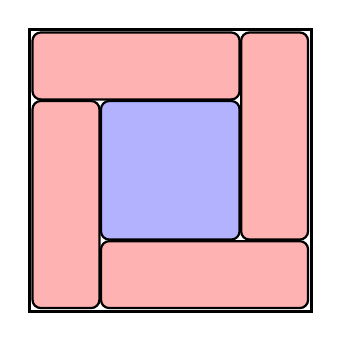
\begin{tikzpicture}[>=latex]
    \def\s{3.5}
    \def\gap{0.85}
    \draw[very thick] (-0.04, -0.04) rectangle (\s + 0.04, \s + 0.04);
    \draw[thick, rounded corners = 3, fill = blue!30] (\gap + 0.02, \gap + 0.02) rectangle
        (\s - \gap - 0.02, \s - \gap - 0.02);
    \draw[thick, rounded corners = 3, fill = red!30] (0, 0) rectangle (\gap, \s - \gap - 0.02);
    \draw[thick, rounded corners = 3, fill = red!30] (0, \s) rectangle (\s - \gap - 0.02, \s - \gap);
    \draw[thick, rounded corners = 3, fill = red!30] (\gap + 0.02, 0) rectangle (\s, \gap);
    \draw[thick, rounded corners = 3, fill = red!30] (\s - \gap, \gap + 0.02) rectangle (\s, \s);
\end{tikzpicture}
 	\caption{}
 	\label{fig:partition-rect}
\end{figure}
	

\subsection{Fooling Set}

Пусть дана матрица некоторой функции. Выберем клетки этой таблицы $a_1, a_2, \ldots, a_n$ так, чтобы
никакие две из них не могли оказаться в одном <<одноцветном>> прямоугольнике, то есть состоящего только
из нулей или только из единиц. Тогда для каждой клетки должен быть свой прямоугольник разбиения. Отсюда
следует, что в дереве протокола должно быть хотя бы $n$ вершин, а высота дерева хотя бы $\log n$. Этот
метод называется \deftext{Fooling Set}.  

Например, его можно применить для функции
$$
    \EQ(x, y) \coloneqq
    \begin{cases}
        1, & x = y,\\
        0, & x \neq y,
    \end{cases}
$$
на строчках длины $m$ мы получим диагональную матрицу $2^m \times 2^m$, и тогда в качестве точек $a_i$
можно выбрать единицы на диагональной матрице. Понятно, что никакие две из них не находятся в одном
одноцветном прямоугольнике. Значит высота коммуникационного дерева хотя бы $\log 2^m = m$.

Похожим образом мы можем доказать нижнюю оценку на функцию $\Disj(x, y)$ на подмножествах множества
$[n]$, которая принимает значение $1$ тогда и только тогда, когда $ x \cap y = \emptyset$. Для всех
множеств $S \in [2^n]$ рассмотрим ячейку матрицы $a_S \coloneqq (S, \overline{S}$). Заметим, что для $S
\neq S'$ ячейки $a_S$ и $a_{S'}$ не могут лежать в одном прямоугольнике, так как иначе в этом
прямоугольнике лежат ячейки $(S, \overline{S'})$, $(S', \overline{S})$, и в одной из них стоит $0$. Из
чего мы можем заключить, что высота коммуникационного дерева хотя бы $\log 2^n = n$.  


\subsection{Игры Карчмера--Вигдерсона}

\begin{definition}
    \deftext{Формульной сложностью} $L(f)$ формулы $f$ будем называть минимальное возможное число листьев
    дерева, вычисляющего эту формулу (в вершинах дерева стоят булевы операции $\vee, \wedge$, а на
    некоторых рёбрах стоят $\neg $).
\end{definition}

\begin{theorem}[Шеннон]
    Существует такая функция $f\colon \{0, 1\}^n \to \{0, 1\}$, что:
    $$
        L(f) \ge \bigO{\frac{2^n}{n}}.
    $$
\end{theorem}

\begin{proof}
    Заметим, что количество функций $f\colon \{0, 1\}^n \to \{0, 1\}$ равно $2^{2^n}$. Посмотрим на
    всевозможные формулы сложности не более, чем $s$. Каждое из них представляет собой двоичное дерево
    с не более, чем $2s - 1$ вершинами, в которых написаны булевы операции, и не более, чем $s$ листьями,
    в которых написаны переменные. Тогда в каждой вершине стоит один из $n + 6$ символов ($n$ переменных и
    $2$ булевых символа с возможными отрицаниями перед ними), а количество деревьев c не более, чем
    $2s - 1$ вершинами, по теореме Кэли не превосходит:
    $$
        (2s - 1)^{2s - 3}(2s - 1) \le (2s)^{2s} \le 2^{4s \log s}.
    $$ 
    Отсюда следует, что количество деревьев сложности не более, чем $s$, не превосходит
    $2^{4s \log s + 2s \log(n + 6)}$. Осталось убедиться, что при $s < \frac{2^n}{10n}$ количество
    деревьев сложности не более, чем $s$ не превосходит количество функций
    $f\colon \{0, 1\}^n \to \{0, 1\}$. Действительно, при $s < \frac{2^n}{10n}$ верно, что
    $2^{4s\log s + 2s \log(n + 6)} < 2^{2^n}$. А значит существует формула, сложность которой хотя бы
    $\frac{2^n}{10n}$.
\end{proof}
    
На данный момент <<самая сложная>> известная <<явная>>, то есть для неё есть алгоритм, считающий её за
полиномиальное время, функция $f$, для которой выполнено $L(f) \geq n^{3 - \varepsilon}$.

Рассмотрим функцию $f\colon \{0, 1\}^n \to \{0, 1\}$. Для $f$ можно рассмотреть следующую
коммуникационную задачу $\KW_f$: Алиса получает число $x \in f^{-1}(1)$, Боб~--- $y \in f^{-1}(0)$. Их
цель~--- найти хотя бы одну позицию $i$, в которой $x_i \ne y_i$. В случае, если таких битов несколько,
то подойдет любой.

\begin{theorem}[Карчмер--Вигдерсон]
    \label{th:KW-theorem}
    Любую формулу для $f$ можно переделать в коммуникационный протокол для $\KW_f$ с таким же деревом и
    обратно. В частности, минимальная глубина формулы для $f$ равна коммуникационной сложности $\KW_f$.
\end{theorem}

\begin{proof}
    Функцию, которую считает гейт формулы $u$, будем обозначать $f_u$; аналогично, прямоугольник,
    соответствующий вершине протокола $v$, будем обозначать $R_v$.
    
    Начнем с <<простой>> части и построим по формуле коммуникационный протокол. Пусть Алиса получила на
    вход строку $x \in f^{-1}(1)$, а Боб строку $y \in f^{-1}(0)$. Назовём гейт формулы $u$
    \deftext{хорошим}, если $f(x) \neq f(y)$.

    Будем строить протокол, начиная с корня дерева формулы. По условию задачи, корень~--- это хорошая
    вершина, целью Алисы и Боба на каждом раунде будет являться поиск хорошего предка. И тогда,
    перемещаясь на каждом раунде в такого предка, Алиса и Боб найдут хороший лист, в котором и будет тот
    вход формулы, на котором строки Алисы и Боба различаются. Таким образом, для того, чтобы завершить
    доказательство, нам достаточно показать, как найти хорошего предка, передав не более одного
    бита. Рассмотрим текущую вершину $u$ с предками $a, b$ (НУО считаем, что $f_u(x) = 1 \wedge f_u(y) =
    0)$. У нас возможны два случая.
    \begin{enumerate}
        \item В вершине $u$ написан значок $\wedge$. Тогда заметим, что $f_a(x) = f_b(x) = 1$, и при этом
            либо $f_a(y) = 0$, либо $f_b(y) = 0$. Таким образом, Боб может однозначно определить, какой
            из предков является хорошим, и сообщить это Алисе, передав один бит.
        \item В вершине $u$ написан значок $\vee$. Тогда заметим, что $f_a(y) = f_b(y) = 0$, и при этом
            либо $f_a(x) = 1$, либо $f_b(x) = 1$. Таким образом, Алиса может однозначно определить, какой
            из предков является хорошим, и сообщить это Бобу, передав один бит.
    \end{enumerate}


    Теперь по протоколу построим формулу. По индукции, начиная с листьев протокола, для каждой вершины
    протокола $v$ мы предъявим формулу для такой функции $f_v$, что $f_v(X_v) = 1$ и $f_v(Y_v) = 0$,
    где $R_v \coloneqq X_v \times Y_v$.

    Рассмотрим лист протокола $\ell$ и заметим, что прямоугольник $R_{\ell} \coloneqq X_{\ell} \times
    Y_{\ell}$ одноцветный, поэтому все строки $x \in X_{\ell}$ отличаются от всех строк $y \in Y_{\ell}$
    в какой-то фиксированной позиции $i_{\ell}$, в частности это означает, что выполнен один из двух
    следующих случаев:
    \begin{itemize}
        \item для всех $x \in X_{\ell}, y \in Y_{\ell}$ бит $x_{i_{\ell}} = 1$ и $y_{i_{\ell}} = 0$,
            тогда мы можем определить $f_{\ell} \coloneqq x_{i_{\ell}}$;
        \item для всех $x \in X_{\ell}, y \in Y_{\ell}$ бит $x_{i_{\ell}} = 0$ и $y_{i_{\ell}} = 1$,
            тогда мы можем определить $f_{\ell} \coloneqq \neg x_{i_{\ell}}$.
    \end{itemize}
    Других случаев не существует, поскольку если найдутся такие $x, x' \in X$, что $x_{i_{\ell}} \neq
    x'_{i_{\ell}}$, то они одновременно не могут отличаться в позиции $i_l$ ни от какого $y$ (случай
    $y_{i_{\ell}} \neq y'_{i_{\ell}}$ аналогичен).

    Построим теперь формулу для функции $f_v$, если у нас уже есть формулы для функций $f_a$ и $f_b$, где
    $a, b$~--- потомки вершины $v$. Заметим, что прямоугольники $R_a$ и $R_b$ получены рассечением
    прямоугольника $R_v$ на две части либо вертикальным, либо горизонтальным сечением. Рассмотрим эти
    случай отдельно и заметим, что:
    \begin{itemize}
        \item если сечение было горизонтальным, то $Y_a = Y_b = Y_v$ и $X_v = X_a \cup X_b$ и в таком
            случае нам подойдет формула $f_v \coloneqq f_a \vee f_b$;
        \item если сечение было вертикальным, то $X_a = X_b = X_v$ и $Y_v = Y_a \cup Y_b$ и в таком
            случае нам подойдет формула $f_v \coloneqq f_a \wedge f_b$.
    \end{itemize}
\end{proof}